%%%%%%%%%%%%%%%%%%%%%%%%%%%%%%%%%%%%%%%%%%%%%%%%%%%%%%%%%%%%%%%%%%%%%%%%%%%%%%%%%%%%%%%%%%%%%
%%									Chapitre 2												%
%%%%%%%%%%%%%%%%%%%%%%%%%%%%%%%%%%%%%%%%%%%%%%%%%%%%%%%%%%%%%%%%%%%%%%%%%%%%%%%%%%%%%%%%%%%%%

\chapter{Les différents métiers au laboratoire SOLEIL}
	\minitoc
	

%%%%%%%%%%%%%%%%%%%%%%%%%%%%%%%%%%%%%%%%%%%%%%%%%%%%%%%%%%%%%%%%%%%%%%%%%%%%%%%%%%%%%%%%%%%%%



% Début du chapitre
			
	

		Pendant mon stage à SOLEIL, j'ai observé les différents métiers qui permettent au synchrotron de fonctionner et aux chercheurs de faire leurs expériences.			

		\section{Ingénieur calcul}
			L'ingénieur calcul vérifie la rigidité des pièces car sous l'effet des variations de température, les métaux se dilatent ou se contractent. Il doit concevoir des pièces pouvant fonctionner dans différentes conditions. Il doit pouvoir estimer les températures pour savoir comment construire les éléments. Pour pouvoir estimer la rigidité des objets, il utilise des méthodes de calculs numériques.
			
			L'ingénieur est spécialiste en calculs scientifiques. Il a une formation Bac+5 en école d'ingénieur. Son salaire est de 2250 euros par mois en tant que débutant et aujourd'hui il gagne 4000 euros par mois. Si il veut évoluer dans son métier, il peut se spécialiser dans certains domaines.
			
			L'avantage de ce métier est qu'il n'y a pas d'horaires décalés car pas de contraintes d'exploitation.  
		
		\section{Coordinateurs expérience}
			Le coordinateur expérience est responsable du bon fonctionnement de chaque ligne de lumière. Il doit pouvoir intervenir dans tous les domaines de la physique. Il doit aussi connaître les gestes de premier secours et savoir utiliser les machines.
			
			Le coordinateur expérience est ausi là pour surveiller la machine. Comme son exploitation est très coûteuse, elle est aussi utilisée  pendant les week-end et la nuit. Le coordinateur doit donc être présent quand les autres personnes ne travaillent pas.
			
			Au synchrotron SOLEIL il y a six coordinateurs expériences. Ils se partagent le travail en trois fois huit heures par journée. Cela veut dire que chaque jour, il y a trois coordinateurs expérience qui travaillent~: un travaille le matin, le deuxième travaille l'après-midi et en fin de soirée et le troisième travaille pendant la nuit. Ils échangent les postes tous les jours (week-end et jours fériés compris). Pour que chacun puisse avoir des vacances, ils sont six.
			
			Les formations pour ce poste sont scientifiques~: il faut un bac scientifique et avoir fait des études supplémentaires en physiques. Il faut parler anglais et connaître les termes spécifiques en anglais, parce qu'au synchrotron SOLEIL, des chercheurs et scientifiques de tous les pays viennent travailler.
			
			Le salaire est d'environ 3500 euros net par mois.

			Le désavantage de ce métier est qu'il faut dormir le jour quand on travaille la nuit. 
		
		\section{Mécaniciens}
			\par Lors de la construction de l'accélérateur d'électrons, les mécaniciens ont installé les pièces et construit la machine. 
			
			\par Maintenant, ils s'occupent de la maintenance de la machine et construisent des pièces avec différentes outils. Ils utilisent la fraiseuse et la tourneuse pour travailler le métal et créer différentes pièces. Ils utilisent aussi une rectifieuse pour lisser les faces, une plieuse pour plier les différents métaux. Les mécaniciens soudent aussi.
			
			\par Leur revenu est entre 1600 et 2000 euros net mensuels. La formation est un apprentissage en école spécialisée, un CAP, un BEP ou un Bac Pro.
		
		\section{Services achats}
			Au sein du service administratif, certaines personnes s'occupent des achats. Pour cela, il y a une assistante, trois acheteurs et deux personnes qui passent les commandes. Les catégories d'achats sont les fournitures, les services, et les travaux.
		
		\section{Videurs}
			 Certaines personnes s'occcupent de vérifier si les tubes sont bien sous vide. En effet les tubes ne doivent pas contenir de molécules d'air autrement les électrons s'entrechoqueraient avec ces molécules ou seraient détournés puis s'écraseraient sur la paroi des tubes et ne pourraient plus servir aux expériences.
			
			\par Pour mettre sous vide, on utilise des pompes à spirales qui aspirent l'air puis l'évacuent vers l'extérieur. On passe de dix puissance vingt-quatre molécules par mètre-cube d'air à dix puissance dix-neuf molécules par mètre-cube. 
			\par On trouve également des molécules sur les parois. Elles peuvent se décoller et dégrader le vide rendant le tube inutilisable pour les expériences. Pour éviter cela, on chauffe les parois de cent degrés celsius à deux-cent degrés celsius pendant environ vingt-quatre heure. Après tout ces processus, il reste dix puissance onze molécules par mètre-cube. 
			\par On utilise également des pompes ioniques ou statiques qui piègent les molécules. Même si le vide n'est pas encore parfait, il est alors suffisant pour mener à bien les expériences car la probabilité d'interaction d'un électron avec une molécule résiduelle est suffisament petite. 

			\par Si on pense qu'il y a une fuite quelque part dans un tube ou une pièce, on utilise un détecteur. On vaporise de l'hélium autour de la pièce et un détecteur nous informe par un graphique si l'hélium a pu entrer dans le tube. Si l'hélium est entré dans le tube il faut réparer la pièce abimée.  
		
		\section{Électronicien et Électrotechnicien}
			Les électroniciens et les électrotechniciens développent, mettent au point et maintiennent les aimants. Parfois ils travaillent pour d'autres pays.
		
		\section{Resources humaines}
			Les personnes travaillant dans le groupe ressources humaines s'occupent des salaires, aident les salariés si ils ont des problèmes, s'occupent de l'embauche des personnels et des stagiaires. Lorsqu'une personne est embauchée, les personnes du groupe ressources humaines constituent un dossier électronique. 

		\section{Chercheurs}
			Les scientifiques travaillent avec les lignes de lumière pour faire des expériences. Ils utilisent la lumière émise par les électrons pour observer des échantillons qu'ils déposent dans la cabane d'expériences. Dans chaque ligne de lumière, les expériences sont différentes. J'ai visité plusieurs lignes de lumières comme MARS, LUCIA, DIFFABS et METROLOGIE.
			
			\par La ligne de lumière MARS a pour but d'étudier des échantillons de matière radioactives. Les personnes qui y travaillent doivent se protéger pour ne pas être irradiées et tomber malade. Si un sachet transportant un élément radioactif se perce, un instrument bippe pour prévenir les personnes du danger. Sur MARS, les scientifiques utilisent des rayons X. Ils vérifient que les échantillons ne sont pas trop dangereux pour l'homme, par exemple pour savoir si les bâtiments contaminés par la radioactivité sont encore utilisables ou non (par exemple pour d'anciennes centrales nucléaires).
			
			\par Sur LUCIA, les scientifiques étudient les matériaux grâce à la spectroscopie.
			
			\par Les scientifiques de la ligne de lumières DIFFABS travaillent sur la cristallographie. 
			
			\par Sur la ligne de lumière METROLOGIE, les scientifiques font de la lithographie. Ils font des gravures avec de la lumière.
			
			\par Pour devenir chercheur dans le domaine de la physique, il faut un Bac S, continuer des études universitaires jusqu'au niveau Master (BAC+5), puis passer un doctorat dans un laboratoire de recherche (BAC+8).



		\begin{figure}
  			\centering
  		 	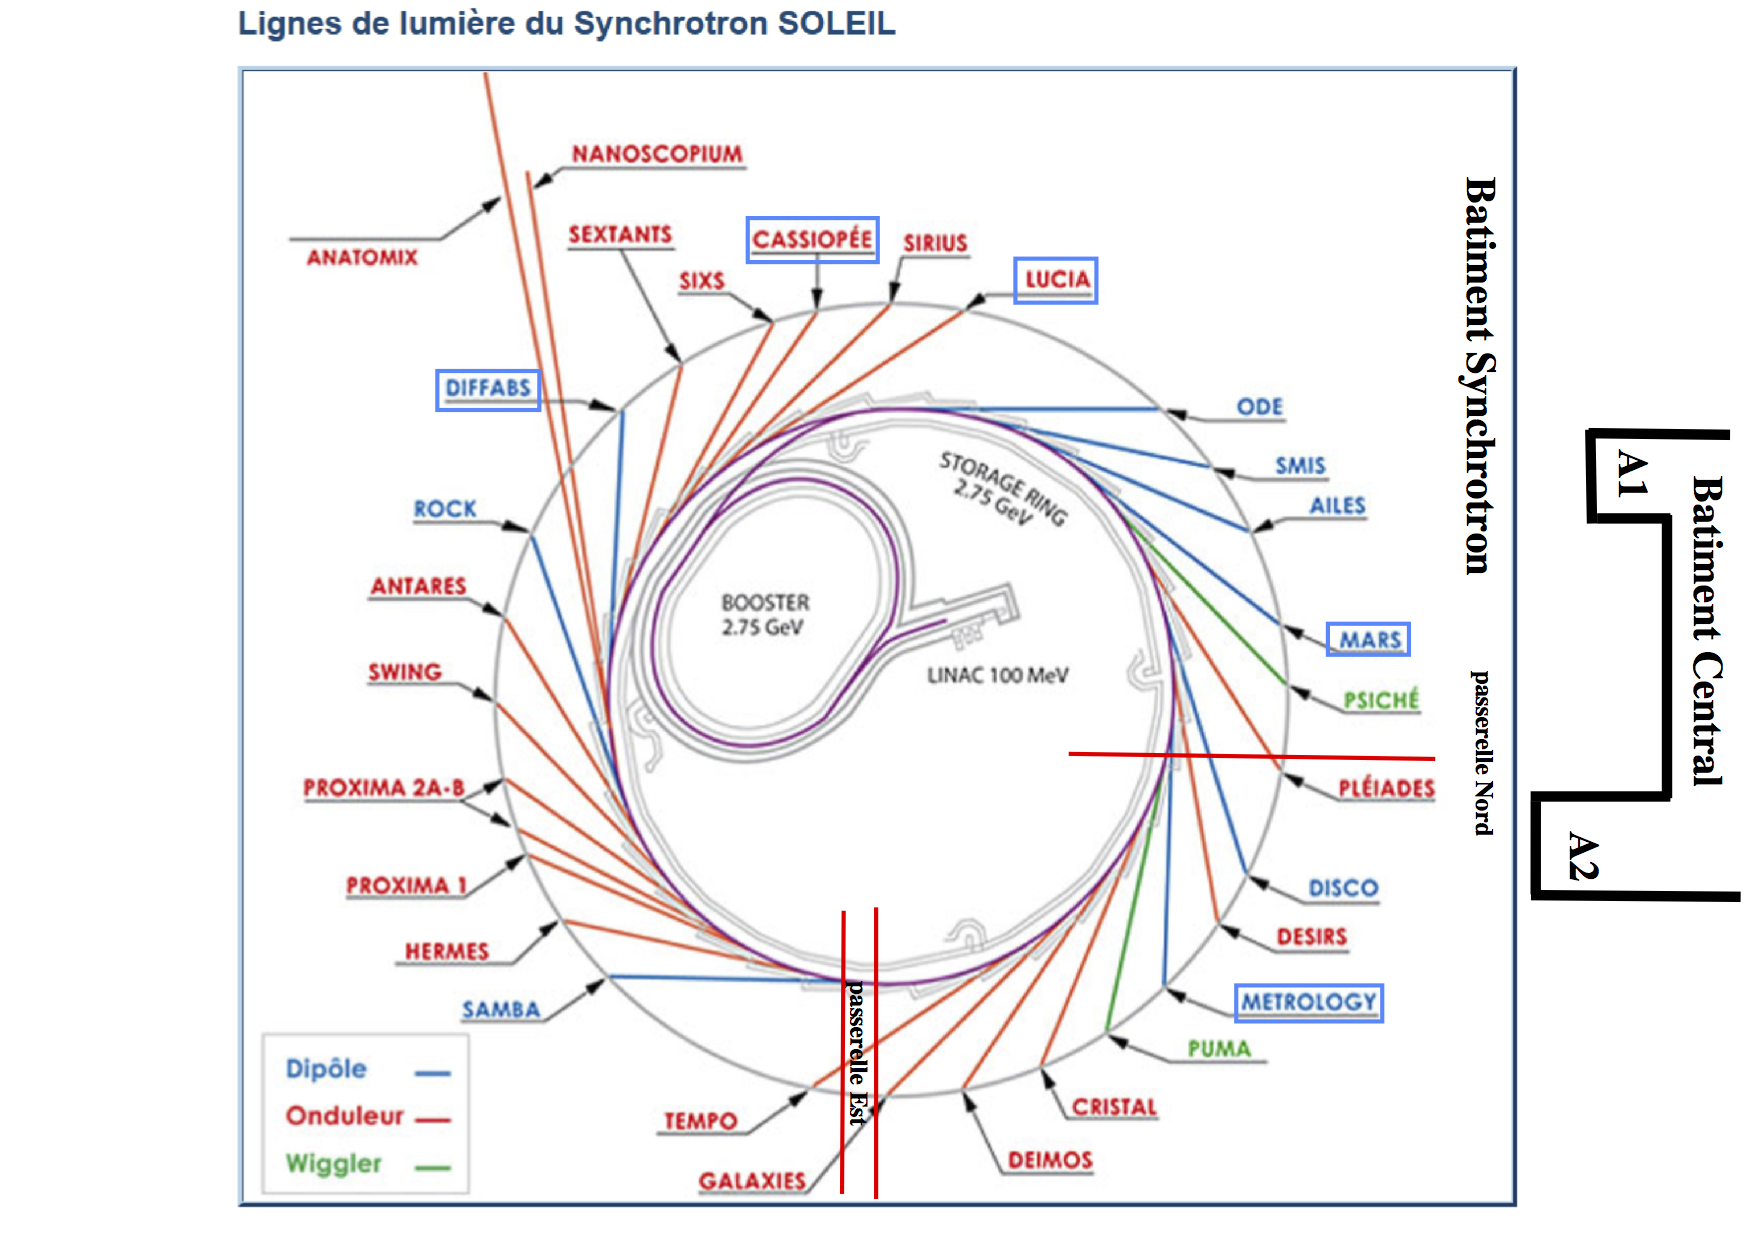
\includegraphics[width=16cm]{Chapitre2/planlignedelumieressoleil}}
  		 	\caption{Lignes de lumière}
		\end{figure}


	
